\section{Modifications related to ViSaG}
\label{sec:modif}
\label{modifications}

This chapter is a review of the modifications made on the prototype (VPOP1) to make a fully functional version of POP-C++ VS for the ViSaG project. The new version includes also the modifications made on POP-C++ for the Secure version (for more information, please refer to "POP-C++ over SSH Tunnel"\cite{popcssh}).

\subsection{Compilation of four different versions of POP-C++}
As POP-C++ could be installed for different usage (cluster, secure, virtual ...), the ability to compile the right version is fundamental. There are four different ways to compile POP-C++ by passing option to the configure script. Here are the four versions : 

\begin{itemize}
\item \textbf{POP-C++} Standard version (cluster, local test...) : configure without options
\item \textbf{POP-C++ S}ecure version (with SSH tunnelling) : configure with the option --enable-secure
\item \textbf{POP-C++ V}irtual version (with worker virtualization - Admin Node only) : configure with the option --enable-virtual
\item \textbf{POP-C++ V}irtual-\textbf{S}ecure version (SSH tunnelling and worker virtualization - for Admin Node only) : configure with the options --enable-virtual --enable-secure
\end{itemize}

\textit{NOTE:} Be aware that all the versions are not fully compatible with each other. For the moment, standard and virtual version can be used together and secure and virtual secure versions can be used together. A compatibility table is available in the document "POP-C++ Virtual-Secure : POP-C++ User and Installation manual add-on"\cite{popc_vs_addon_manual}.\s

\begin{figure}[ht]
	\caption{POP-C++ Global Services}
  	\centering
	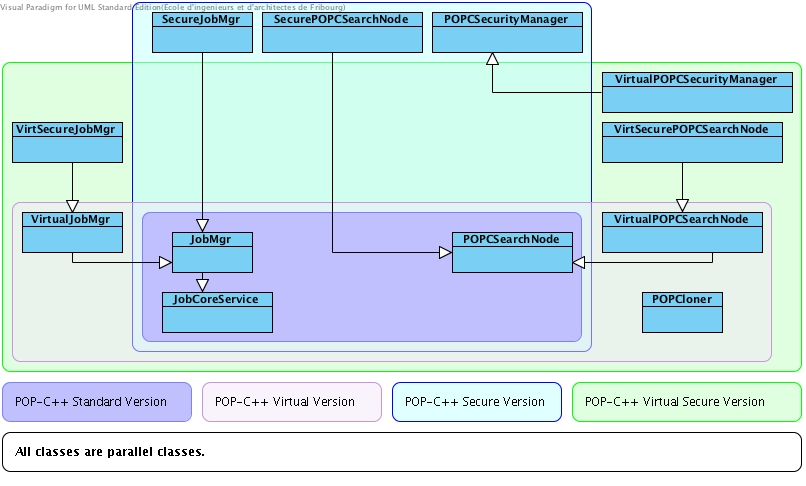
\includegraphics[width=1.0\textwidth]{./pic/global_service_cd.jpg}
	\label{fig:global_service_cd}
\end{figure}

To make this compilation possible, the POP-C++ Global Services has been specialized with new classes. Figure \ref{fig:global_service_cd} shows the new class diagram of the POP-C++ Global Services in each version.\s

All the modifications related to the VS version are now made in the VirtSecureJobMgr, VirtualJobMgr, VirtSecurePOPCSearchNode, VirtualPOPCSearchNode and VirtualPOPCSecurityManager. These modifications will let the future versions of POP-C++ evolve easily one relative to another.\s

To configuration script will create one of the four follwoing variables : STANDARDSUPPORT, VIRTSUPPORT, SECURESUPPORT, VIRTSECURESUPPORT. The created variable is used in the input makefile (Makefile.am) to define to right compilation process. \s

After any modification in the configure.ac file, it is very important to run the following command to generate the new configure script. 
\begin{lstlisting}
autoreconf
\end{lstlisting}\s

\textbf{Files created:} ./lib/virtual\_jobmgr.ph, ./lib/virtual\_jobmgr.cc, ./lib/virtual\_secure\_jobmgr.ph, ./lib/virtual\_secure\_jobmgr.cc, ./lib/virtual\_popc\_search\_node.ph, ./lib/virtual\_popc\_search\_node.cc, ./lib/virtual\_secure\_popc\_search\_node.ph, ./lib/virtual\_secure\_popc\_search\_node.cc, ./lib/virtual\_popc\_secu rity\_manager.ph, ./lib/virtual\_popc\_security\_manager.cc,
 ./services/secure\_jobmgr\_obj.cc,  ./services/virtual\_secure\_jobmgr\_obj.cc,  ./services/secure\_popc\_search\_node\_obj.cc,  ./services/virtual\_secure\_popc \_search\_node\_obj.cc,  ./services/virtual\_popc\_security\_manager\_obj.cc \s

\textbf{Files modified:} ./configure.ac, ./lib/jobmgr.ph, ./lib/jobmgr.cc, ./lib/popc\_search\_node.ph, ./lib/Makefile.am, ./lib/interface.cc, ./script/popc\_setup.in, ./services/Makefile.am\s



%
% HYPERVISOR INFORMATION
%
\pagebreak
\subsection{Hypervisor information}
Instead of being stored in environment variables, the information relative to the hypervisor connection have been stored in the Virtual JobMgr configuration file. This file is located under \textit{POPC\_LOCATION}/etc/virtu- al.conf. The installation script writes the information directly into this configuration file instead of writing them into a script that initialize the environment variables. \s

The VirtualJobMgr constructor retrieves all the information stored in the configuration file. These values are stored into attributes and used when needed.\s

\textbf{Files modified: } ./lib/virtual\_jobmgr.cc, ./lib/virtual\_jobmgr.ph, ./script/popc\_setup.in\s

\subsubsection{Hiding password in POP-C++ Virtual Configuration}
The configuration file used in the virtual version of POP-C++ contains some sensible data. These data must be encrypted to avoid unwanted usage of it. To do this task, we choose to encrypt the whole configuration file. This section explains the different algorithm available to this this job and the one we choose in POP-C++ VS.\s


\textbf{Encryption/Decryption algorithm}\\
There are two main category of encryption/decryption algorithm. These two categories are explained below:

\begin{itemize}
\item \textbf{Symmetric encryption}: using one key two encrypt and decrypt. Figure \ref{fig:symmetric_algo}A shows the encryption/decryption process of a symmetric algorithm.
\item \textbf{Asymmetric encryption}: using a pair of private/public keys. One key is used to encrypt the message and the second to decrypt it. Figure \ref{fig:asymmetric_algo}B shows the encryption/decryption process of an asymmetric algorithm. In this kind of encryption, we could even use an external dongle that manages the encryption and the decryption of the file. 
\end{itemize}
 
 \begin{figure}[ht]
	\caption{Symmetric and Asymmetric encryption algorithm}
  	\centering
	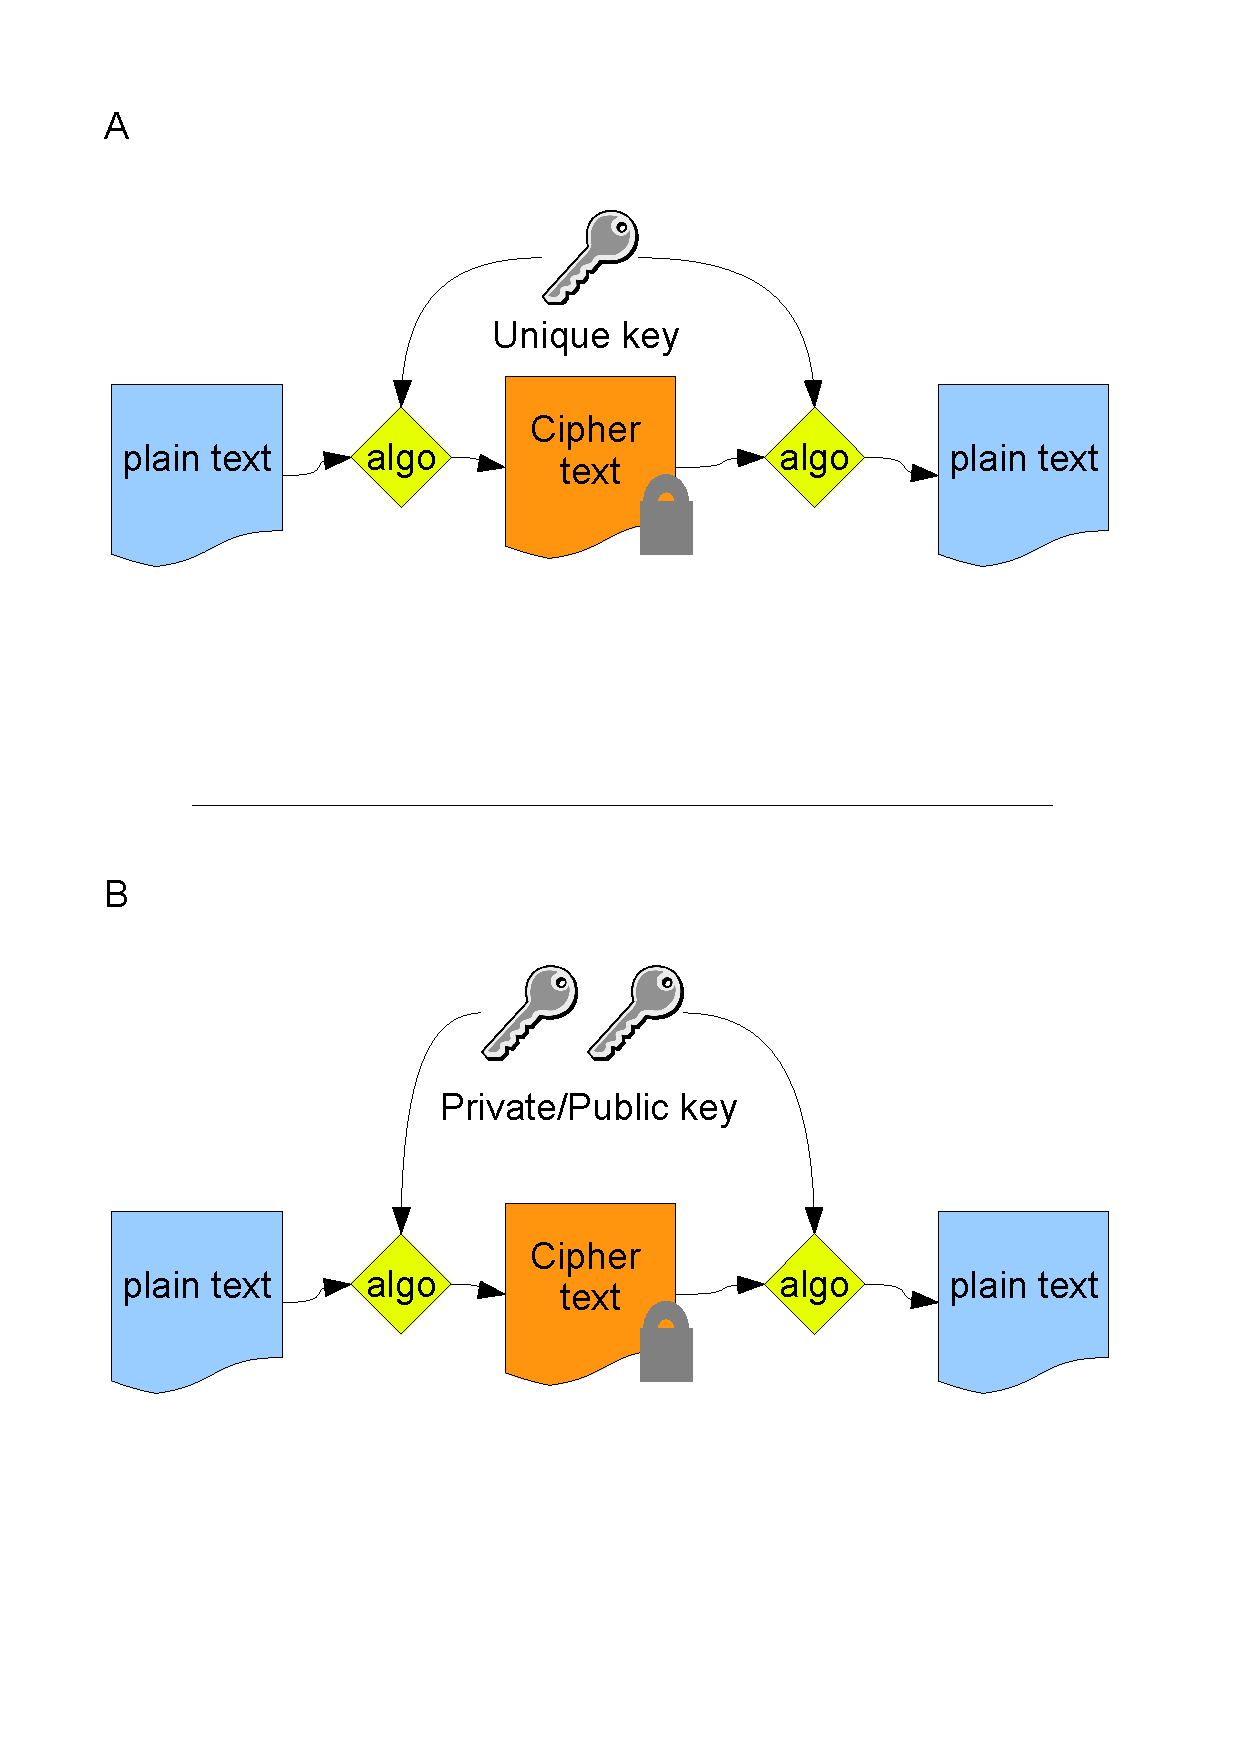
\includegraphics[width=0.7\textwidth]{./pic/encrypt_algo.pdf}
	\label{fig:asymmetric_algo}
\end{figure}

\pagebreak
\textbf{Algorithm used in POP-C++ VS}\\
To encrypt the configuration file used in the POP-C++ VS, we choose to use the AES (rijndael) algorithm. The first step is to generate a key and cipher the information about the virtual configuration. Figure \ref{fig:cipher1} shows this first step. During the compilation of POP-C++, a key is generated and integrated to the executable of POP-C++. A small program is compiled to be able to cipher the information about the virtual configuration during the installation of POP-C++. This program is called \textbf{popcipher}. As shown in Figure \ref{fig:cipher1}, the JobMgr configuration file is not encrypted at all. Only the virtual configuration file is processed by \textbf{popcipher} as this file includes some important passwords. 

\begin{figure}[ht]
	\caption{POP-C++ Virtual Configuration - Cipher - Step 1}
  	\centering
	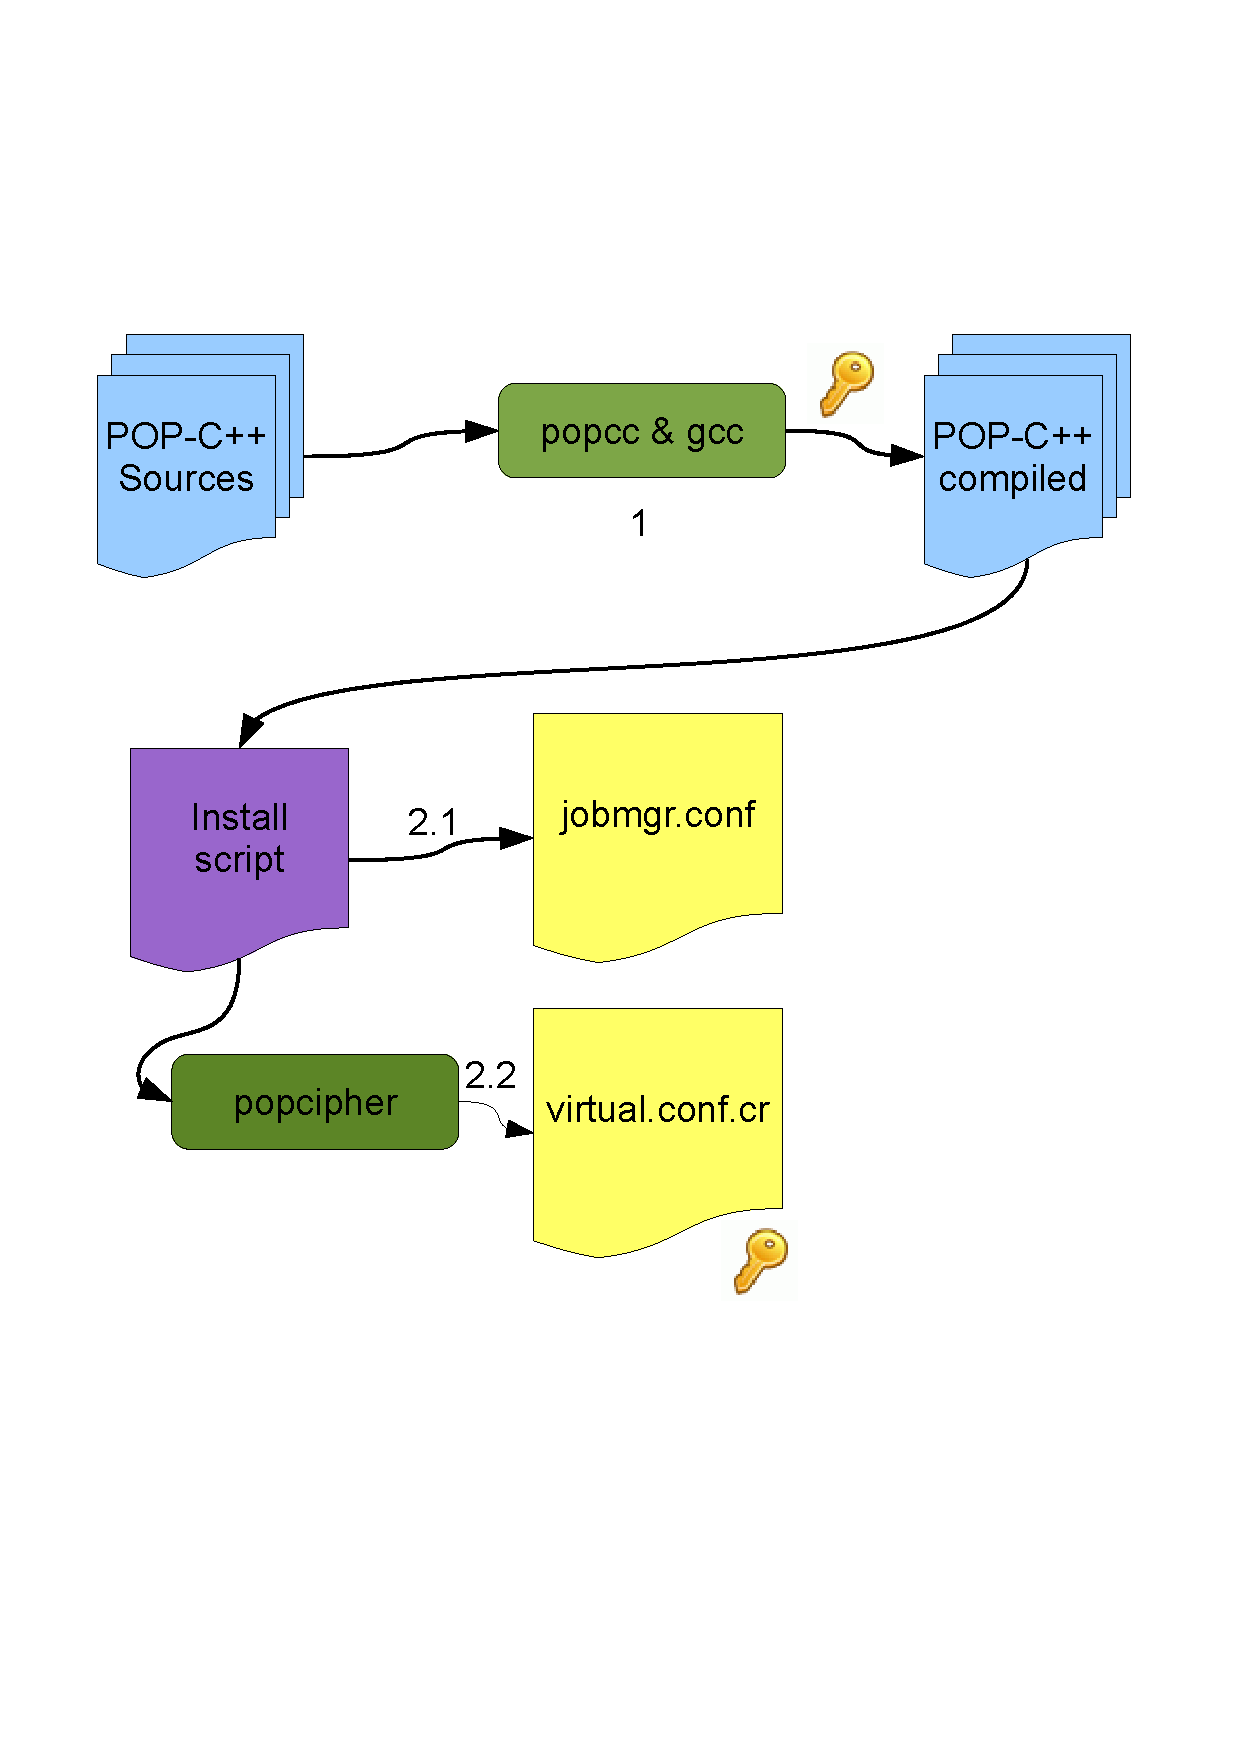
\includegraphics[width=0.5\textwidth]{./pic/cipher1.pdf}
	\label{fig:cipher1}
\end{figure}


Once the virtual configuration file is encrypted, POP-C++ need a way to read these information. Figure \ref{fig:cipher2} shows the starts of the POP-C++ Global Services. Once the Virtual Secure JobMgr (VirtSecureJobMgr) is stared by the "SXXpopc" script, this object will read the virtual.conf.ci file. This object has the ability to decipher this file as during the compilation of POP-C+, the generated key has been included in its executable. The VirtSecureJobMgr deciphers the virtual.conf.ci file and uses its information directly in memory. All the information located in the jobmgr.conf file are read as usual as they are all in clear. \s
\begin{figure}[ht]
	\caption{POP-C++ Virtual Configuration - Cipher - Step 2}
  	\centering
	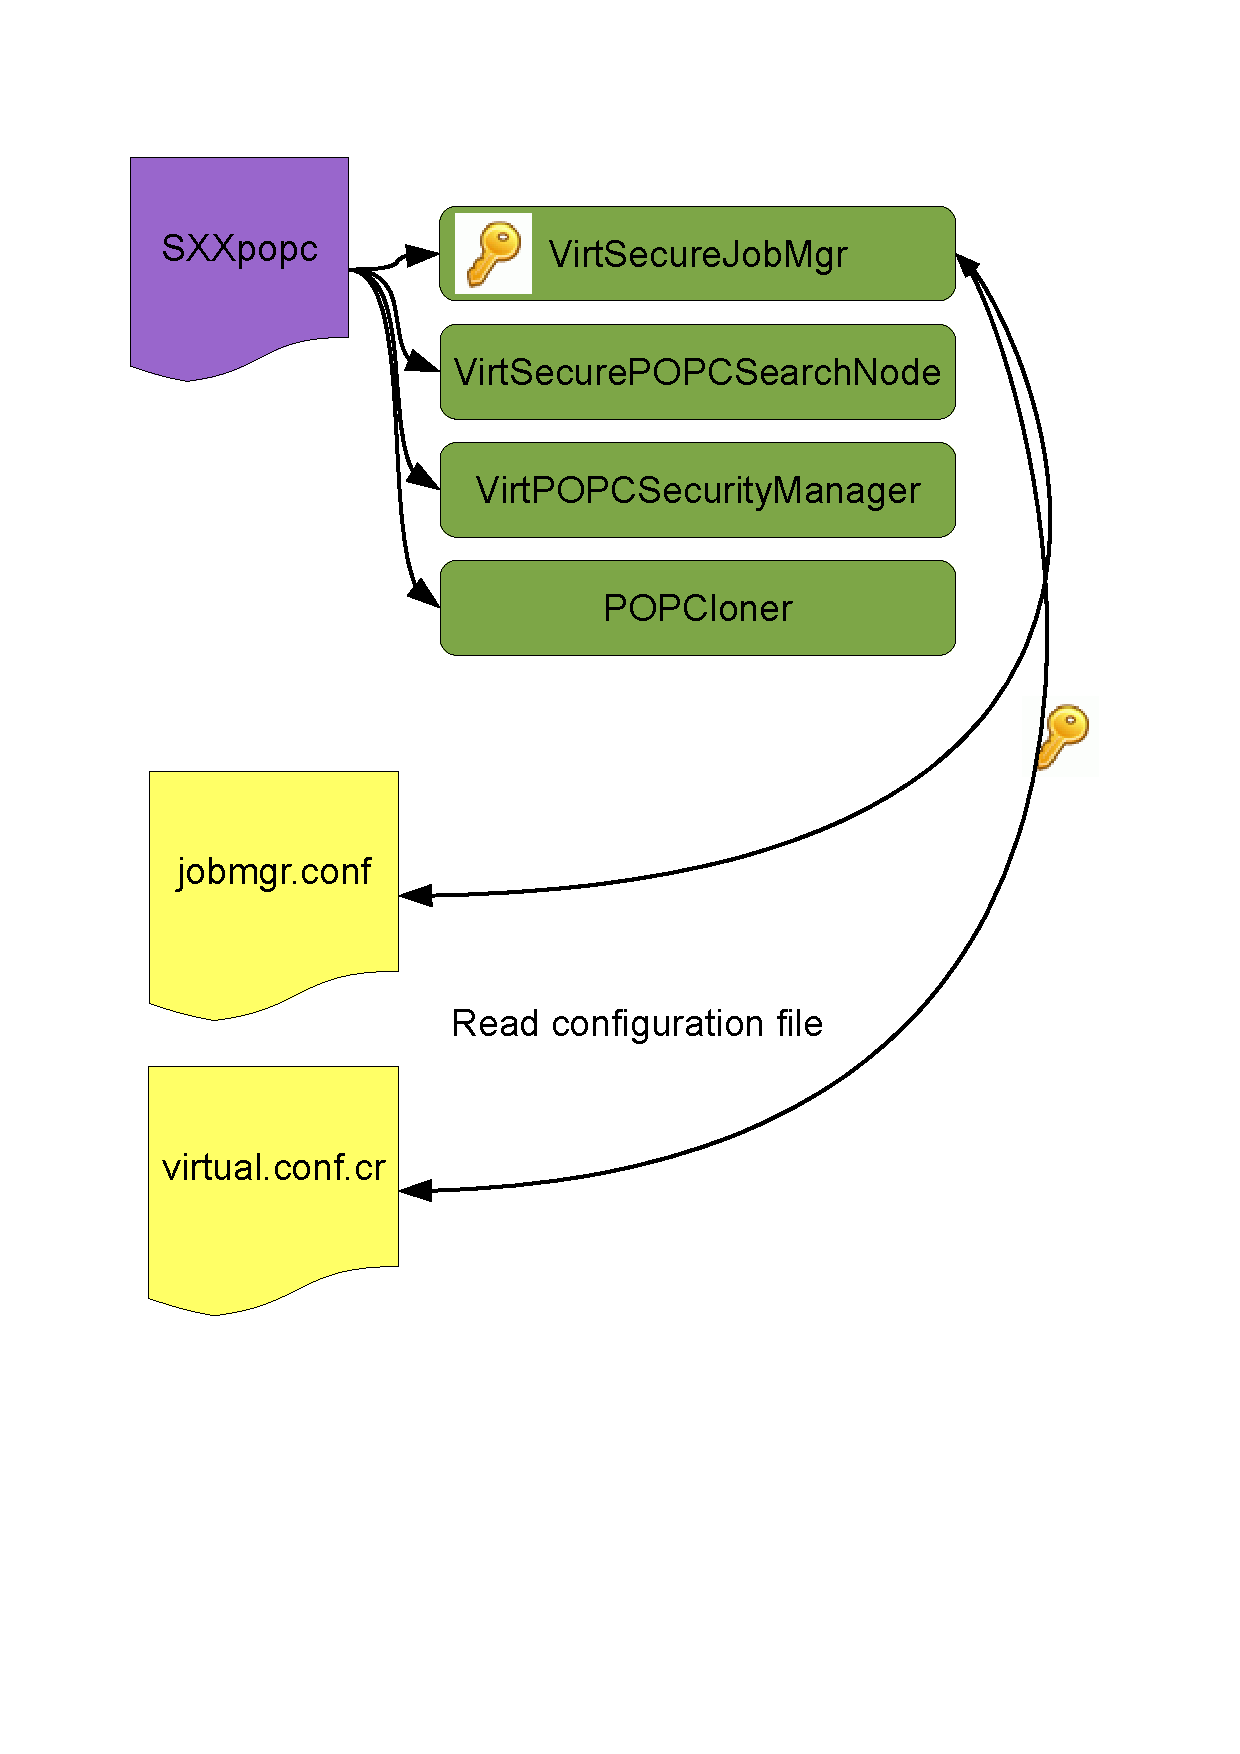
\includegraphics[width=0.5\textwidth]{./pic/cipher2.pdf}
	\label{fig:cipher2}
\end{figure}


\pagebreak
%
% POP APPLICATION IDENTIFIER
%
\subsection{POP Application Identifier}
The AppCoreService has been modified to generate the POP Application ID. This ID is generated in the constructor of this object. The "Request" object has also been modified to include this ID. Just before launching the resource discovery, the JobMgr will contact the AppCoreService to know the POPAppID and set it in the request. The other JobMgrs contacted will know for which application a request has been launched. \s

For more information about the POP Application Identifier, please refer to the document "POP-C++ over SSH Tunnel"\cite{popcssh} in section 7.1.\s

In addition to these modifications, the reservation process must also include the POPAppID and the RequestID. The "struct Resources" defined in \textbf{./lib/jobmgr.ph} have been modified to include the POPAppID and the RequestID. The "Reserve" method must now accept the POPAppId and the RequestID as parameters. At this point, the JobMgr has all the information to manage the different Worker VM.\s

\textbf{Files modified : } ./include/request.h, ./include/Makefile.am, ./lib/request.cc, ./lib/appservice.ph, ./lib/appservice.cc, ./lib/jobmgr.cc, ./lib/Makefile.am\s

\textbf{Files added : } ./include/popwayback.h, ./lib/popwayback.cc



\subsection{Modification of the VPopCWrapper}
\label{lb:wrapper}
The VPopCWrapper was designed to use only one worker VM at the same time. To be able to manage more than one worker, the VPopCWrapper has been changed. A POPvm object has been created to encapsulate all the information relative to a Worker VM. This object is then passed to some of the wrapper method. Each POPvm object has a pointer to its own domain (pointer of domain is a notion introduced by libvirt). This pointer is saved and then any operation of the wrapper can be executed on this VM. \s

The POPvm object encapsulates the following information at the moment : \s
\begin{enumerate}
\item The VM name (displayName)
\item The VM configuration file (VMX file on ESXi)
\item The VM volume (datastore on ESXi)
\item The VM OS
\item The VM clean snapshot
\item The VM IP address
\item The POPAppID (if the VM is reserved)
\item The VM PKI 
\item The VM state (free, reserved, busy)
\end{enumerate} 


The VPopCWrapper interface has been changed to use this new object and be more flexible. The new interface looks as follows : 
\begin{itemize}
\item int \_popc\_connectOpenAuth(string uri, string user, string password);
\item int \_popc\_connectClose();
\item virDomainPtr \_popc\_domainLookupByName(string domName);
\item int \_popc\_domainState(POPvm \&vm, string* state);
\item long long \_popc\_nodeGetFreeMemory();
\item int \_popc\_nodeGetinfo(nodeInfo* info);
\item int \_popc\_domainSnapshotNum(POPvm \&vm);
\item int \_popc\_domainSnapshotListNames(POPvm \&vm, string names[], unsigned short len);
\item int \_popc\_domainRevertToSnapshot(POPvm \&vm, string snapshotName);
\item int \_popc\_domainRevertToOldestSnapshot(POPvm \&vm);
\item int \_popc\_domainSnapshotCreate(POPvm \&vm, string name, string description);
\item int \_popc\_domainSnapshotDelete(POPvm \&vm, string snapshotName, bool removeChildren = false);
\item int \_popc\_domainSetMemory(POPvm \&vm, unsigned long memoryInKb);
\item int \_popc\_domainSetMaxMemory(POPvm \&vm, unsigned long memoryInKb);
\item long \_popc\_domainGetMaxMemory(POPvm \&vm);
\item int \_popc\_domainShutdown(POPvm \&vm);
\item int \_popc\_domainSuspend(POPvm \&vm);
\item int \_popc\_domainResume(POPvm \&vm);
\item const string \_popc\_domainGetMac(POPvm \&vm);
\item int \_popc\_domainGetIpAddress(POPvm \&vm);
\item int \_popc\_domainIsConnected(string domName="");
\item int \_popc\_sendLocalPublicKey(POPvm \&vm);
\item int \_popc\_sendPublicKey(POPvm \&vm, POPString pki);
\item int \_popc\_getLocalPublicKey(POPvm \&vm);
\item int \_popc\_domainClone(POPvm \&original, POPString baseName, int suffix, paroc\_accesspoint clonerAP);
\item int \_popc\_domainWaitingForTools(POPvm \&vm);
\item const string \_popc\_getError();
\end{itemize}

In addition to the modifications above, some of the methods in the ESX implementation of the wrapper have been modified to use the VIX API instead of launching shell command. These changes are explained in Section \ref{lb:vix}.\s

A basic implementation of the VPopCWrapper is done in with the object POPWrapper. This object implements all the methods that can be implemented with libvirt. The ESXWrapper extends the POPWrapper and re-implements only the needed methods. Figure \ref{fig:wrapper_cd} shows the class diagram of wrapper objects. 

\begin{figure}[ht]
	\caption{Virtual Wrapper - Class Diagram}
  	\centering
	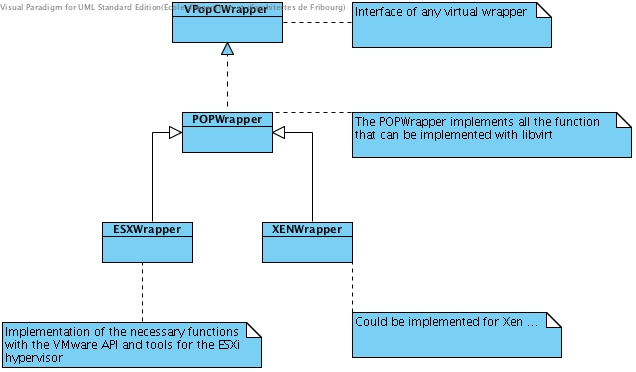
\includegraphics[width=1.0\textwidth]{./pic/wrapper_cd.jpg}
	\label{fig:wrapper_cd}
\end{figure}


%
% VIX COMPILATION
%

\pagebreak
\subsection{POP-C++ and VIX}
\label{lb:vix}
As said in Section \ref{lb:wrapper}, the VIX API is used for some methods in the ESX implementation of the wrapper. These methods were using shell command to do their tasks. It's way better to use API call to perform those actions. Libvirt could one day implement the needed functions available in VIX. If so, the ESX implementation should be modified. 

\subsubsection{Include VIX in the compilation process}

All the necessary modifications done in the configuration script and makefile to include VIX in the compilation process are listed below.\s

\textbf{File: configure.ac:}\\
As the VIX API does not install a ".pc" file for the pkg\_config function. We have to declare the \_CFLAGS and the \_LIBS marcos for VIX. The lines below have been added to the "configure.ac" file. \s

\begin{lstlisting}
VIX_CFLAGS="-lvixAllProducts -ldl"
VIX_LIBS="-I/usr/include/vmware-vix"
AM_SUBST([VIX_CFLAGS])
AM_SUBST([VIX_LIBS])
\end{lstlisting}\s

\textbf{File: ./lib/Makefile.am:}\\
The input Makefile located in the "lib" directory must also be modified. The VIX macros must be added to the macro "AM\_CXXFLAGS". \s

\begin{lstlisting}
AM_CXXFLAGS= OTHER_FLAGS $(VIX_CFLAGS) $(VIX_LIBS)
\end{lstlisting}\s

With those modifications, POP-C++ can now be compiled with the VMware VIX API. \s

\textit{NOTE:} The VIX API must be installed on the machine which compile POP-C++ in its Virtual or Virtual-Secure version. 


\subsubsection{Using VIX to get the worker VM IP address}
The VIX API allow us to read some properties on the guest VM. This ability is used to read the IP address of the guest VM. The process is going as follows:

\begin{enumerate}
\item Connect to the hypervisor (VixHost\_Connect())
\item Get a pointer to the VM (VixHost\_OpenVM())
\item Power on the VM if not running (VixVM\_PowerOn())
\item Waiting for the VMware tools to be ready (VixVM\_WaitForToolsInGuest())
\item Read the variable "ip" (VixVM\_ReadVariable())
\end{enumerate}\s

\textit{NOTE:} For the full code, please see the file ./lib/ESXWrapper.cc method "\_popc\_domainGetIpAddress(POPvm \&vm);"

\subsubsection{Using VIX to send and write the admin VM public key on worker VM}
The VIX API has two very interesting functions that allow us to send a file on the worker VM and to execute a command on the worker VM. To transfer the Admin VM PKI to the Worker VM, we can send the public key file and write it in the authorized\_keys file on the Worker VM by executing a shell command. The process to do this using VIX is going as follows: \s

\begin{enumerate}
\item Connect to the hypervisor (VixHost\_Connect())
\item Get a pointer to the VM (VixHost\_OpenVM())
\item Power on the VM if not running (VixVM\_PowerOn())
\item Waiting for the VMware tools to be ready (VixVM\_WaitForToolsInGuest())
\item Login in the guest VM (VixVM\_LoginInGuest())
\item Copy the Admin VM public key file to the guest VM (VixVM\_CopyFileFromHostToGuest())
\item Execute a command on the guest to write the key (VixVM\_RunProgramInGuest())
\end{enumerate}\s

\textit{NOTE:} For the full code, please see the file ./lib/ESXWrapper.cc method "\_popc\_sendLocalPublicKey(POPvm \&vm);"

\subsubsection{Using VIX to execute a ping on the Worker VM}
As the Worker VM is reverted from a snapshot, its saved IP address could be used by another computer when reverted. To be sure to have a valid IP address before executing jobs on the Worker VM, the guest will ping the Admin VM. This procedure will change the guest IP address if this one is invalid on the network. To execute this action, the wrapper uses the VIX API as well. The process is going as follows: 

\begin{enumerate}
\item Connect to the hypervisor (VixHost\_Connect())
\item Get a pointer to the VM (VixHost\_OpenVM())
\item Power on the VM if not running (VixVM\_PowerOn())
\item Waiting for the VMware tools to be ready (VixVM\_WaitForToolsInGuest())
\item Login in the guest VM (VixVM\_LoginInGuest())
\item Execute a ping on the guest to contact the Admin VM (VixVM\_RunProgramInGuest())
\end{enumerate}\s

\textit{NOTE:} For the full code, please see the file ./lib/ESXWrapper.cc method "\_popc\_reversePing(POPvm \&vm, POPString ipAdress);"


\pagebreak
\subsection{Cloning function implementation}
As no built-in cloning function is currently implemented either in the VIX API or in libvirt, this function has been implemented from scratch. Cloning a VM takes quite some time. Due to that, a parallel object will be in charge of the whole process and let the others Global Services do their respective tasks. The POPCloner object is launched at the Global Services start up in the Virtual and Virtual-Secure version. This object is initialized with the ESXi hypervisor information.\s

When the Admin VM needs to launch a cloning process, a free Worker VM will be reserved as the original VM. This original VM can be used to clone more than one VM. The Admin VM will do a call to the POPCloner and gives the information relative to the orginal VM. The original VM will be busy during the whole process. Once the cloning process is done, the new VM will be added to the list of managed VM and the original VM will be freed. Unfortunately, the cloning process needs several proprietary tools from VMware. Here is the list of those tools : \s

\begin{itemize}
\item VMware VIX API 1.10.2 or later
\item VMware CLI 4.1 or later
\item VMware tools 8.3.2 or later
\end{itemize}\s


The cloning process is detailed below and each action associated with the needed tool/command.

\begin{enumerate}
\item Create a new POPvm object with the information of the new VM.
\item Check if the original is suspended or running and shut it down if it's the case. The original VM \textbf{must} be shutdown to perform the cloning actions (VIX).
\item Retrieve the configuration file (.vmx) of the original VM (vmware-cmd).
\item Create the new folder for the cloned VM (vifs).
\item List all the files in the original folder and filter them (vifs).
\item Copying files from the original to the new created folder (vmkfstools and vifs).
\subitem The .vmx file is read and a new one is created for the new VM.
\item Register the cloned VM (vmware-cmd).
\item Remove useless temporary files
\item Write the VM information in the Virtual JobMgr configuration file. 
\item Start and stop the cloned VM (VIX). This step is fundamental to be able to retrieve the VM with libvirt. 
\item Add the new VM in the list of usable VM (POP-C++ call to the JobMgr).
\end{enumerate}

\textit{NOTE:} For the full code, please see the file ./lib/popcloner.cc.

\textbf{On going development}\\
Even this function is fully functional, we are currently trying to implement this process directly into the libvirt library. As it is still under development, no information can be given now. 

%\subsection{Requirements}
%To be able to run the POP-C++ Virtual version, the following requirements must be fulfilled:

%\begin{center}
%\begin{tabular}{|p{1.8cm}|p{3.3cm}|p{2.7cm}|p{2.6cm}|p{1.5cm}|p{1.5cm}|}
%\hline
%\textbf{VM Type} & \textbf{POP-C++ version}	& \textbf{VMware tools} & \textbf{VMware CLI} & \textbf{VIX} & \textbf{libvirt}\\ \hline
%Admin & Virtual Secure & X & >= 4.1 & >= 10.1 & >= 0.8.5\\ \hline
%Worker & Secure & X & - & - &- \\ \hline
%\end{tabular}
%\end{center}\s

%\begin{itemize}


%\item VMware ESXi 4.1 or later must be installed as the hypervisor.
%\item The VMware tools 8.3.2 build-257589 or later must be installed on the worker VM and on the Admin VM.
%\item The VIX API 1.10 or later must be installed on the admin VM.
%\item libvirt 0.8.3 or later must be installed on the admin VM.
%\end{itemize} 


\pagebreak
\subsection{Reservation process}
The original reservation process of POP-C++ does not take into consideration the VM. To be able to reserve a VM for a specific POP-C++ Application (POPAppID), the "Reserve()" method has been reimplemented for the Virtual and Virtual-Secure JobMgr. Figure \ref{fig:flowchart_reservation} shows a flowchart of the reservation process for both Virtual and Virtual-Secure version. \s

\begin{figure}[ht]
	\caption{Reservation process}
  	\centering
	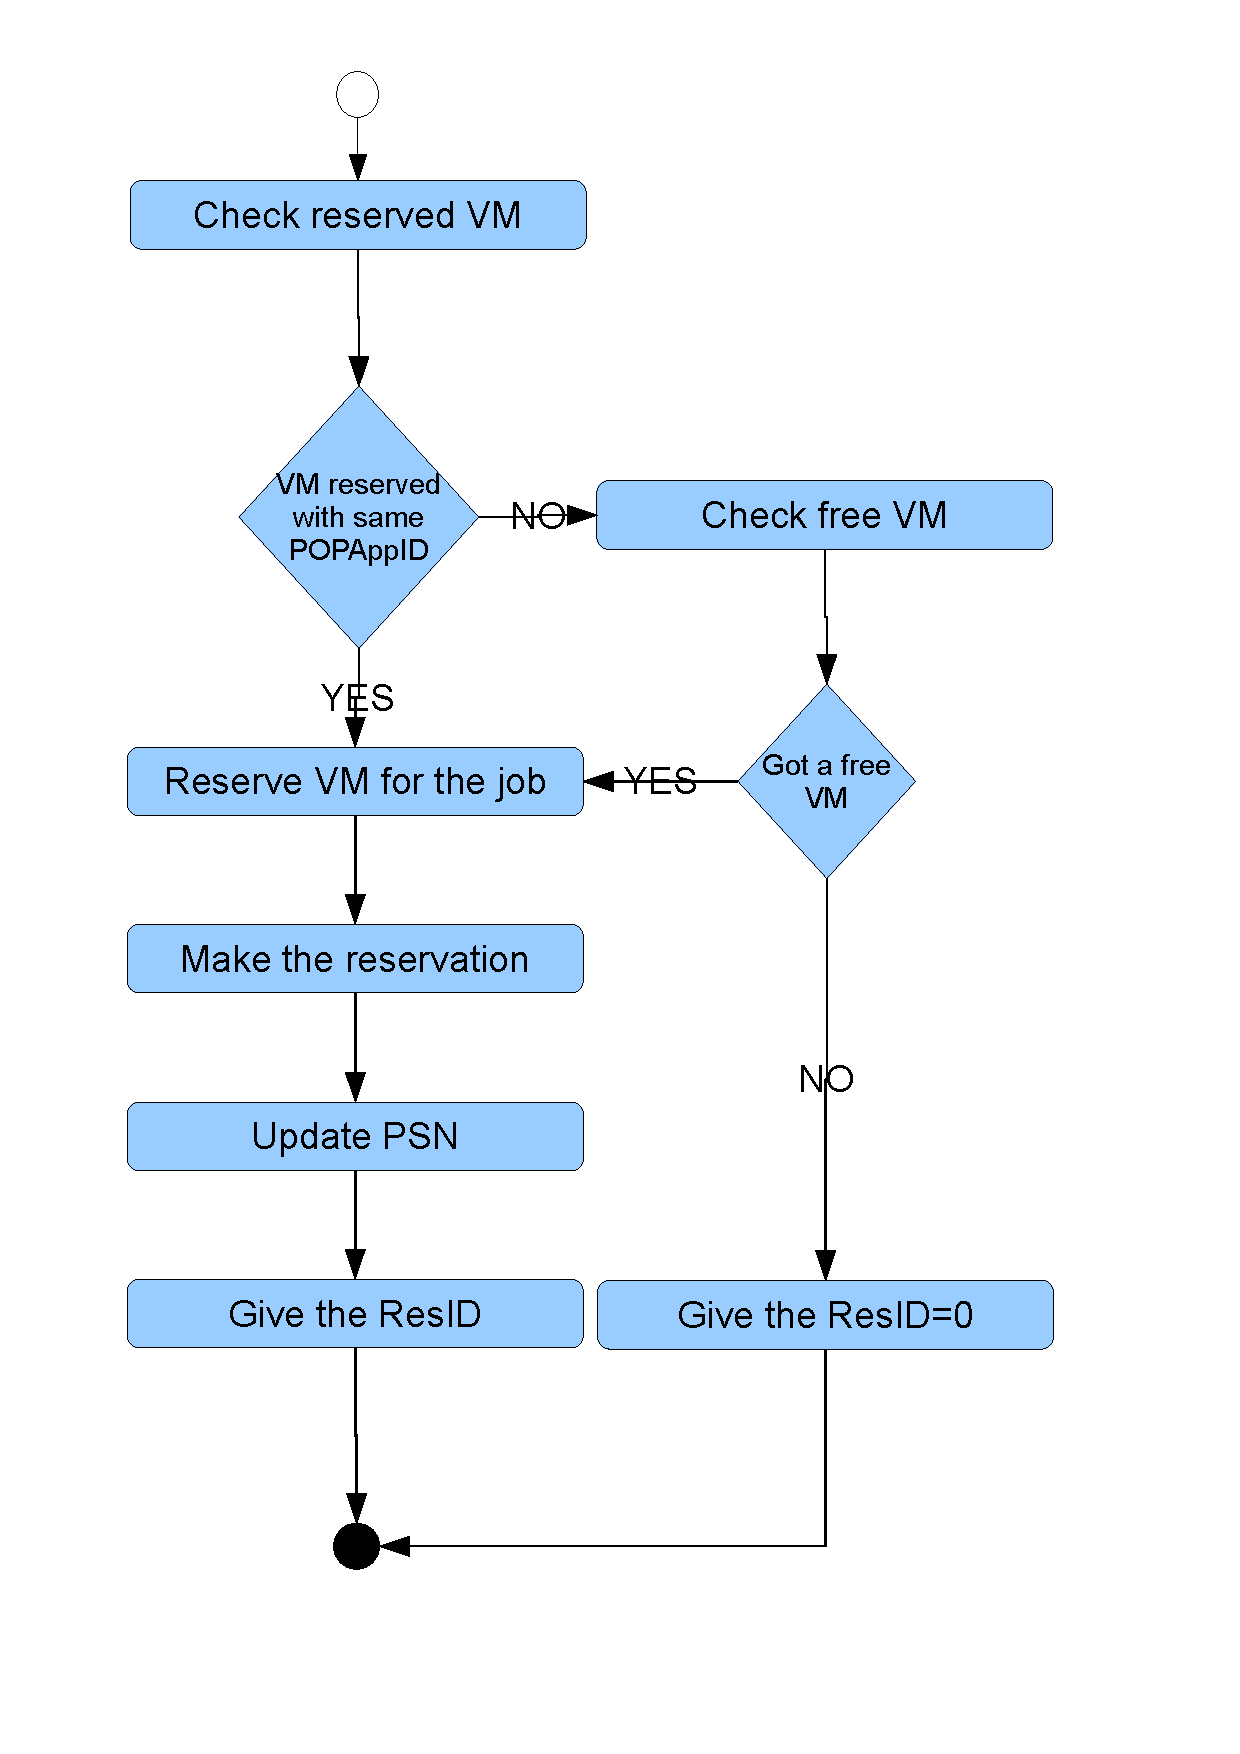
\includegraphics[scale=0.5]{./pic/reserve_vm.pdf}
	\label{fig:flowchart_reservation}
\end{figure}

\pagebreak
\subsection{Preparing a VM to execute a Job}
As POP-C++ is now Virtual and Secure, the preparation of the VM to execute a job is a little bit different. Figure \ref{fig:flowchart_preparation} shows the flowchart of the VM preparation before the job execution.

\begin{figure}[ht]
	\caption{VM Preparation}
  	\centering
	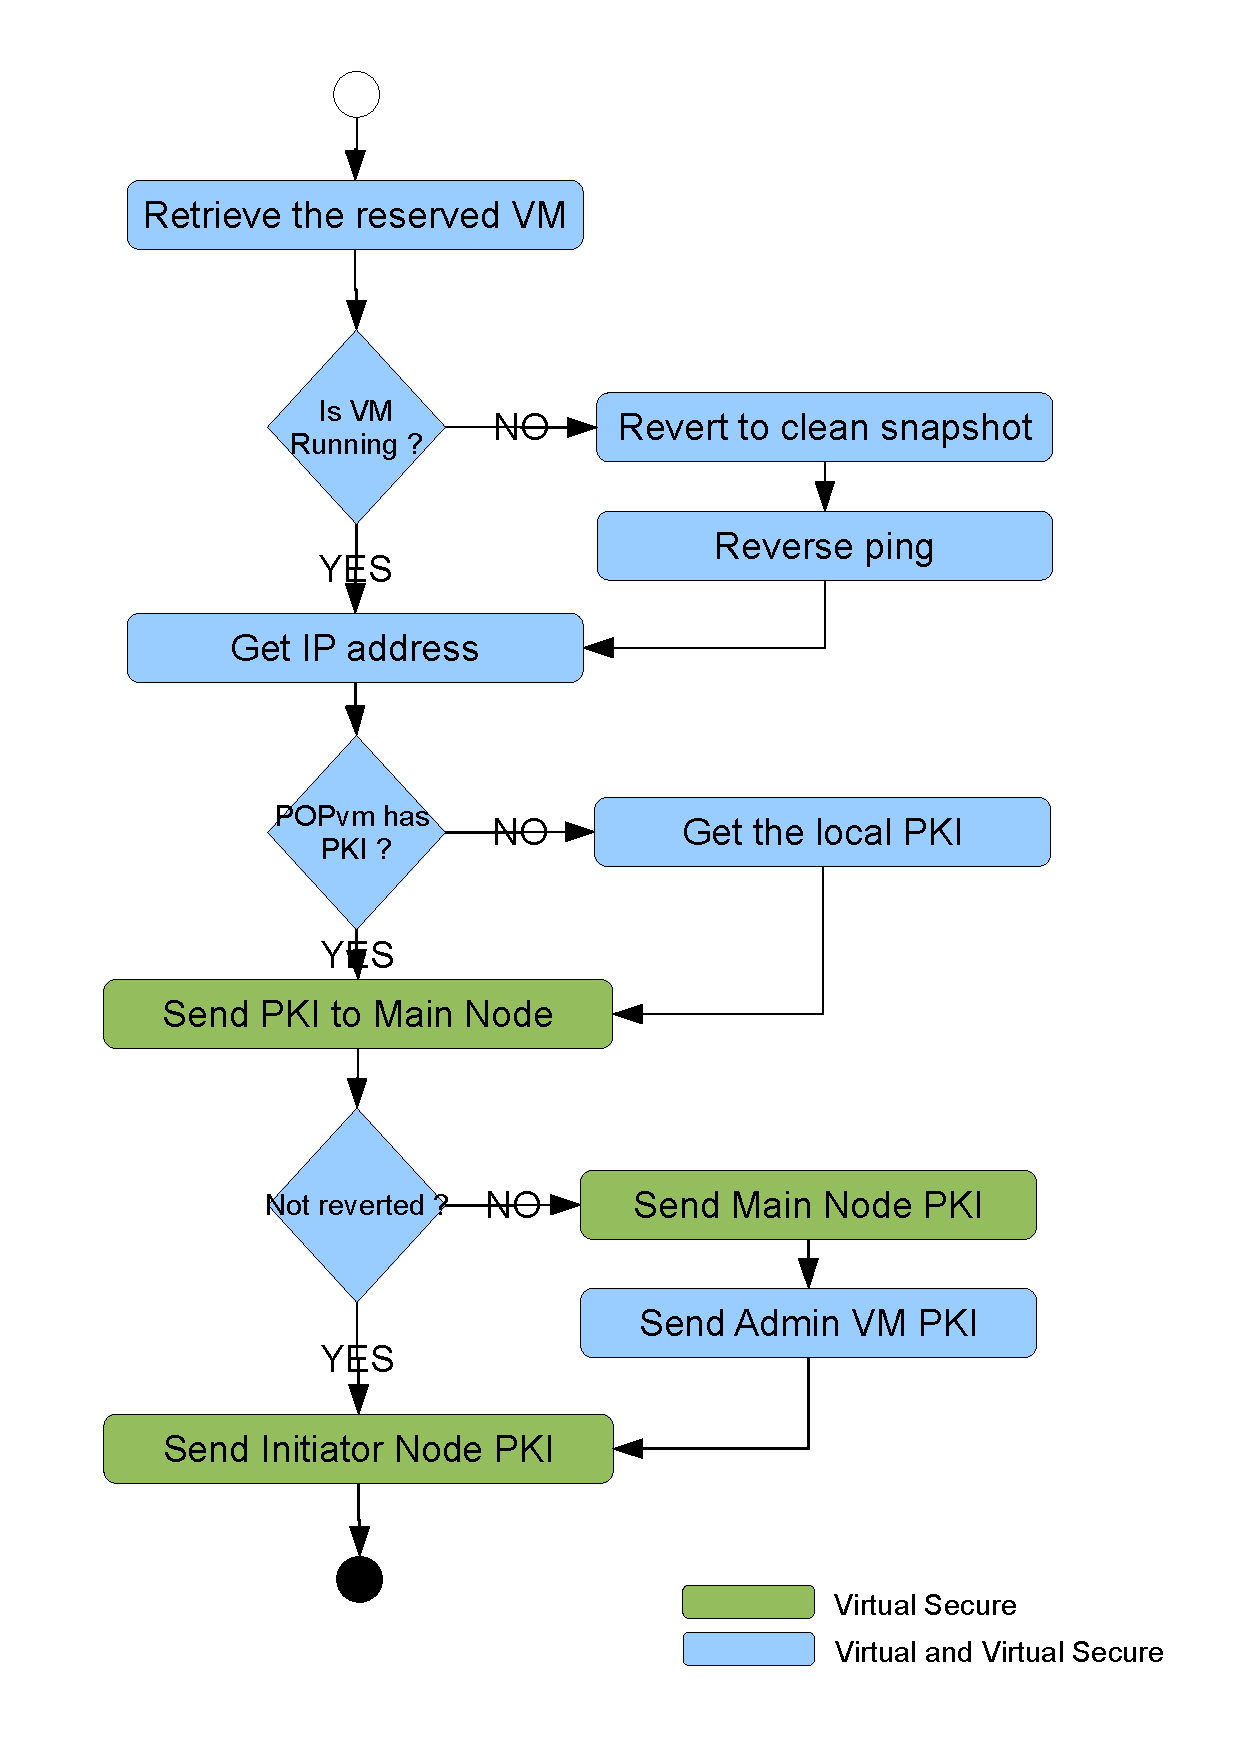
\includegraphics[scale=0.5]{./pic/prepare_vm.pdf}
	\label{fig:flowchart_preparation}
\end{figure}

\pagebreak
\subsection{How to know the Global Services that start an object}
A Worker VM do not have Global Services running on it. When an object is created from another object located on the Worker VM, the interface of this worker needs to know which Global Services has created its broker. This information is fundamental to use the key routing process implemented in the POP-C++ Security Manager as the creator node is the node that will write and send the PKIs. This information is known by the JobMgr just after the resource discovery. To be able to give this information back to the Interface, the method "CreateObject()" of the JobCoreService has been changed a little bit. Here is the new signature of this method. \s

\begin{lstlisting}
sync conc virtual int CreateObject(paroc_accesspoint &localservice, const 
paroc_string &objname, const paroc_od &od, int howmany, [in, out, 
size=howmany] paroc_accesspoint* jobcontacts, int howmany2, [in, out, 
size=howmany2] paroc_accesspoint* remotejobcontacts);
\end{lstlisting}\s

The array "remotejobcontacts" will hold the JobMgr access point that created the object as the array "jobcontacts" hold the access point to the object itself. \s

\textit{NOTE:} The parameter "howmany2" is not mandatory in pure POP-C++ as "howmany" could be used for the second array size. This parameter has been added to keep the compatibility with POP-Java. 


\subsection{Virtual POP-C++ Security Manager}
The POP-C++ Security Manager (PSM) developed in "POP-C++ over SSH Tunnel" is not able to manage a "virtual node" with an Admin VM and some Worker VM. To manage the security of the virtual node, the Virtual POP-C++ Security Manager has been developed. This parallel object inherits from the orginal PSM. \s

In POP-C++ VS, the VirtualPOPCSecurityManager (VPSM) works as a router for the PKI. This parallel object will receive request from others nodes in the GRID but also from the Worker VM associated on its own node. With the POPAppID, the VPSM is able to operate a kind of key routing. This chapter explains the modifications done for this routing process. 

\subsubsection{Add new mapping for Request PKI}
When the Admin VM sends a resource discovery request, all the possible resources will answer with their respective PKI. Unfortunately, the VM that will execute this job is maybe not defined yet. To be able to send the PKI of the chosen resource the the VM, a new mapping has been added in the Virtual PSM. This mapping maps a combination of the POPAppID and the ReqID with the PKI. \s

When a node receives a resource discovery request, it saves the PKI in the mapping. If this node is asked to execute the job, the PKI will be retrieved and sent to the VM.\s

\textbf{Files modified: } ./lib/virtual\_popc\_security\_manager.ph, ./lib/virtual\_popc\_security\_manager.cc, ./lib/virtual\_secure\_popc\_search\_node.cc

\subsubsection{Write the key on a VM}
When a key reaches the PSM, this key must be written on the right VM. As each running Worker VM is attached with a POPAppID, it's easy to find the right VM to write a key if we know the POPAppID associated with this key. \s

Once the VM is retrieved, the VPopCWrapper method "\_popc\_sendPublicKey(POPvm \&vm, POPString pki);" is used to write the key on the Worker VM.\s

\textbf{Files modified:} ./include/VPopCWrapper.h, ./include/ESXWrapper.h, ./lib/ESXWrapper.cc, ./lib/virtual\_popc\_security\_manager.ph, ./lib/virtual\_popc\_security\_manager.cc


\subsection{Application ending}
The POP-C++ runtime must handle the end of a POP-C++ application. The application services destruction can inform the of the end of a POP-C++ application. Once the destructor of the AppCoreService will be called, a call will be propagated to the JobMgr's method "ApplicationEnd(POPString popAppId, bool initiator)". This method will just remove the associated reservation in the standard version. In the Virtual and Virtual-Secure version, this method will suspend any VM reserved for this POPAppID. \s

\textbf{Files modified:} ./lib/appservice.cc, ./lib/jobmgr.ph, ./lib/jobmgr.cc, ./lib/virtual\_jobmgr.ph, ./lib/virtual\_jobmgr.cc


\subsection{Unique starting Worker VM}
As we are able to clone VM, the assumption of a unique worker VM at first start-up is made. On the first start-up, depending on the configuration entered by the user during the installation, some VM can be cloned. This new VM will not appear in the virtual configuration file as we can find them at global services start-up. \s

To be able to do this task, the first VM must respect an important rule. The name of the first worker VM must finish with \textbf{\_worker1}.


\subsection{Using valgrind to detect memory leaks}
Valgrind is a set of tools to detect incorrect memory management in a program. We try to run the POP-C++ Global Services through valgrind to remove any possible leaks or incorrect memory management. \s

\textbf{Running the Interface-side with valgrind}\\
As POP-C++ program are divided into several parts, each part must be run with valgrind. For the Interface-side, the "popcrun" script must be modified to included the valgrind command and options. Here are the modifications made to run the Interface-side with valgrind : \s

\begin{lstlisting}
cmd="valgrind --log-file=/tmp/$PROG$$ $PROG $args -initparoc 
-appservicecode=${MYAPPSERVICE} ${MY_PROXY} -codeconf=${PATHCONF}
/${FILECONF} -jobservice=${MYJOBSERVICE} ${localFlag}"
\end{lstlisting}\s

Some leaks have been detected by using valgrind but not all of them are currently corrected. The results below is the last error to be corrected. 

\begin{lstlisting}
==19039== Syscall param write(buf) points to uninitialised byte(s)
==19039==    at 0x4062523: __write_nocancel (syscall-template.S:82)
==19039==    by 0x80ACE12: paroc_buffer_raw::Send(paroc_combox&, 
   paroc_connection*) (buffer_raw.cc:412)
==19039==    by 0x809F325: paroc_interface::paroc_Dispatch(paroc_buffer*) 
   (interface.cc:1167)
==19039==    by 0x808C0F3: AppCoreService::_paroc_Construct(paroc_string 
   const&, bool, paroc_string const&) (_paroc3_appservice.ph.cc:28309)
==19039==    by 0x808C5C4: AppCoreService::AppCoreService(paroc_string 
   const&, bool, paroc_string const&) (_paroc3_appservice.ph.cc:28291)
==19039==    by 0x80923C7: paroc_system::CreateAppCoreService(char*) 
   (system.cc:477)
==19039==    by 0x80931B3: paroc_system::Initialize(int*, char***) 
   (system.cc:374)
==19039==    by 0x8091F0A: main (paroc_infmain.std.cc:53)
==19039==  Address 0x430f971 is 281 bytes inside a block of size 
   1,044 alloc'd
==19039==    at 0x4025BD3: malloc (vg_replace_malloc.c:236)
==19039==    by 0x4025C5D: realloc (vg_replace_malloc.c:525)
==19039==    by 0x809881F: paroc_array<char>::SetSize(int) 
   (paroc_array.h:156)
==19039==    by 0x80ACCB2: paroc_buffer_raw::Reset() (buffer_raw.cc:30)
==19039==    by 0x80ACFEA: paroc_buffer_raw::paroc_buffer_raw() 
   (buffer_raw.cc:19)
==19039==    by 0x80AD11C: paroc_buffer_raw_factory::CreateBuffer() 
   (buffer_raw_factory.cc:23)
==19039==    by 0x809FCAF: paroc_interface::Encoding(paroc_string) 
   (interface.cc:800)
==19039==    by 0x80A0089: paroc_interface::NegotiateEncoding(
   paroc_string&, paroc_string&) (interface.cc:886)
==19039==    by 0x80A223B: paroc_interface::Bind(char const*) 
   (interface.cc:606)
==19039==    by 0x80A294F: paroc_interface::Bind(paroc_accesspoint const&) 
   (interface.cc:480)
==19039==    by 0x80A4ACF: paroc_interface::Allocate() (interface.cc:444)
==19039==    by 0x808C5A6: AppCoreService::AppCoreService(paroc_string 
   const&, bool, paroc_string const&) (_paroc3_appservice.ph.cc:28290)
\end{lstlisting}



\textbf{Running the Broker-side with valgrind}\\
To run the Broker side with valgrind, we need to change the 
To run the other side of a parallel object using valgrind, the execution of a POP-C++ application was set to manual. In this state, the POP-C++ runtime just print the command used to run the parallel object on the other node. By modifying this command, we are able to run the parallel object broker-side with valgrind. \s

The result of this execution presents no leaks in memory. 
\s

%####################################
%
% GENERAL MODIFICATION ON POP-C++
%
%####################################
\pagebreak
\section{General modifications}
\label{sec:gen_mod}
This chapter regroups all the modifications made on POP-C++ in general. Some of these modifications have been made to fix bugs and some to enhance to possibilities of POP-C++ in all versions. 

\subsection{Update the POP-C++ Search Node resource information}
Currently, the POP-C++ Search Node (PSN) is not updated when a reservation is made on the node. To fix this bug, the PSN has now two additional methods to add a job and to remove a job. With this update, the PSN can directly refuse a resource discovery and not send a response and refuse the reservation later.\s

These methods increase or decrease the resources of the PSN and the number of job currently executed on the node. Here are the signature of these two methods : \s
\begin{lstlisting}
sync seq void addJob(float power, float memorySize, float bandwidth);
sync seq void removeJob(float power, float memorySize, float bandwidth, 
     int nbJob);
\end{lstlisting}

To reduce the number of call to the PSN, the removing method is called once for all the application. 
